\chapter{Dati, Modelli e i Loro Limiti}
\begin{flushright}\small\textit{Lezione 4 -- 16/03/2026 -- G\'eron, Cap.\ 1 (cont.)}\end{flushright}

\section{Ricapitolo: la regressione lineare e la matematica del modello}

La \textbf{regressione lineare} è più antica sia del Machine Learning che dell'Intelligenza Artificiale. Se ci troviamo di fronte a un problema lineare, i dati possono essere rappresentati tramite una tendenza (trend). Mettendo in relazione il PIL pro capite con la soddisfazione di vita, si osserva che all'aumentare del PIL la soddisfazione cresce -- comportamento linearmente crescente.

Ricordiamo l'equazione del modello (già vista nella lezione precedente):
\[
\hat{y} = \theta_0 + \theta_1 \cdot x
\]
che non è altro che l'equazione classica della retta $y = q + mx$, con $\theta_0$ intercetta e $\theta_1$ pendenza. Il grafico seguente mostra tre possibili rette sugli stessi dati:

\begin{center}
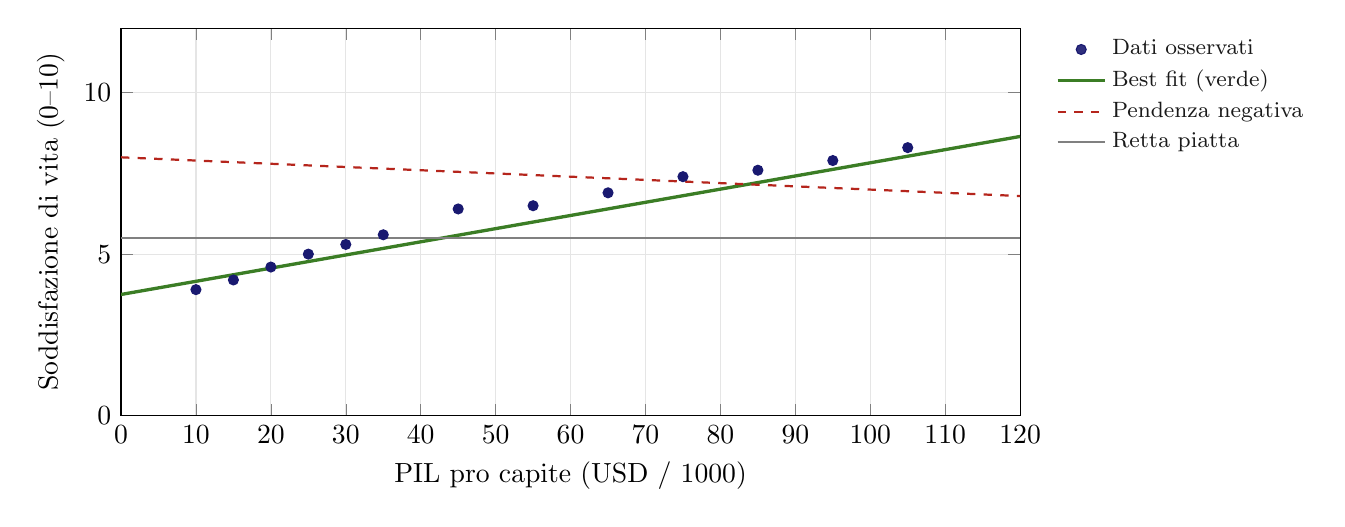
\begin{tikzpicture}
\begin{axis}[
    width=13cm, height=6.5cm,
    xlabel={PIL pro capite (USD / 1000)},
    ylabel={Soddisfazione di vita (0--10)},
    xmin=0, xmax=120, ymin=0, ymax=12,
    grid=major, grid style={gray!20},
    legend pos=outer north east,
    legend style={font=\footnotesize, cells={anchor=west}, 
                  legend columns=1, draw=none, fill=white, fill opacity=0.9},
    legend cell align={left}
]
\addplot[only marks, mark=*, mark size=1.8pt, MidnightBlue] coordinates {
    (10,3.9)(15,4.2)(20,4.6)(25,5.0)(30,5.3)
    (35,5.6)(45,6.4)(55,6.5)(65,6.9)(75,7.4)
    (85,7.6)(95,7.9)(105,8.3)
};
\addlegendentry{Dati osservati}
\addplot[domain=0:120, samples=2, very thick, OliveGreen] {3.75 + 0.0408*x};
\addlegendentry{Best fit (verde)}
\addplot[domain=0:120, samples=2, thick, BrickRed, dashed] {8 - 0.01*x};
\addlegendentry{Pendenza negativa}
\addplot[domain=0:120, samples=2, thick, gray] {5.5};
\addlegendentry{Retta piatta}
\end{axis}
\end{tikzpicture}
\end{center}

\begin{itemize}
    \item \textbf{Verde (pendenza negativa)}: più un paese è ricco, meno le persone sarebbero soddisfatte -- contraddice i dati.
    \item \textbf{Rosso (retta piatta)}: nessuna relazione tra PIL e soddisfazione -- inutile.
    \item \textbf{Blu (best fit)}: segue il trend ascendente dei dati sperimentali. Non passa per ogni singolo punto, ma rappresenta la \textbf{tendenza generale migliore}.
\end{itemize}

\subsection{Come si trovano i parametri ottimali?}

I parametri $\theta_0$ e $\theta_1$ si identificano minimizzando una \textbf{funzione di costo}, tipicamente l'\textbf{MSE} (Mean Squared Error), che misura la distanza media al quadrato tra le previsioni del modello e i valori reali. Minore è l'errore complessivo, migliore è l'approssimazione.

\begin{exbox}[Analogia matematica]
Come nei problemi di ottimizzazione del liceo -- trovare il rettangolo inscritto in una circonferenza con area massima, o il triangolo circoscritto con area minima -- si calcolano le soluzioni ottime ponendo a zero la derivata prima. Nel caso della regressione lineare, essendo un problema con 2 variabili ($\theta_0, \theta_1$), si calcolano \textbf{2 derivate parziali} e si pongono uguali a zero. 

Tuttavia, questa è una soluzione di \textbf{compromesso}: forzare la retta a passare per un punto specifico altera le distanze da tutti gli altri punti.
\end{exbox}


Questo problema ha due soluzioni algoritmiche:
\begin{itemize}
    \item \textbf{Normal Equation}: soluzione analitica chiusa -- calcola direttamente i parametri ottimali con un'operazione matriciale. Efficiente per dataset piccoli.
    \item \textbf{Gradient Descent (discesa del gradiente)}: soluzione iterativa -- parte da parametri casuali e li aggiorna gradualmente nella direzione che riduce l'errore.
\end{itemize}

Con i parametri ottimali $\theta_0 = 3{,}75$ e $\theta_1 = 6{,}78 \times 10^{-5}$, la retta risultante è:
\[
\text{soddisfazione} = 3{,}75 + 6{,}78 \times 10^{-5} \cdot \text{PIL}
\]

\begin{exbox}[Esempio numerico: fissare la soddisfazione e trovare il PIL]
Voglio scoprire quale PIL pro capite corrisponde a una soddisfazione di vita alta ($\hat{y} = 9$):
\[
9 = 3{,}75 + 6{,}78 \times 10^{-5} \cdot x
\quad\Rightarrow\quad
x = \frac{9 - 3{,}75}{6{,}78 \times 10^{-5}} \approx 77\,434 \text{ USD}
\]
Nota: l'asse $x$ del grafico è in USD / 1000, quindi questa scala dilatata è necessaria per evitare che la retta sembri piatta a occhio.
\end{exbox}

\subsection{E se il problema NON è lineare?}

Se i dati seguono un andamento quadratico ($y = ax^2 + b$), si può usare un \textbf{trucco matematico}: sostituire $t = x^2$ e trasformare l'equazione in $y = at + b$, ora lineare. Si risolve con la normale regressione lineare, poi si ritrasforma il risultato.

\begin{center}
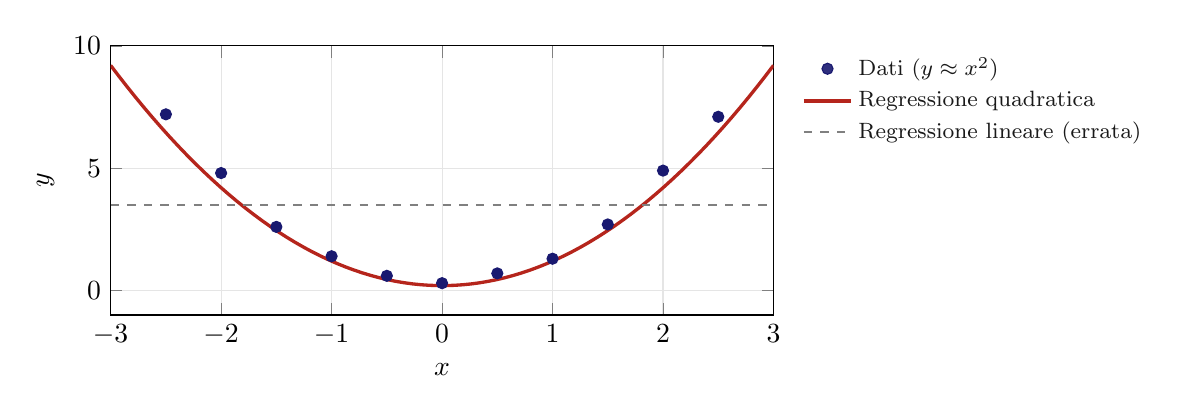
\begin{tikzpicture}
\begin{axis}[
    width=10cm, height=5cm,
    xlabel={$x$}, ylabel={$y$},
    xmin=-3, xmax=3, ymin=-1, ymax=10,
    grid=major, grid style={gray!20},
    legend pos=outer north east,
    legend style={font=\footnotesize, cells={anchor=west}, 
                  legend columns=1, draw=none, fill=white, fill opacity=0.9},
    legend cell align={left}
]
\addplot[only marks, mark=*, mark size=2pt, MidnightBlue] coordinates {
    (-2.5,7.2)(-2,4.8)(-1.5,2.6)(-1,1.4)(-0.5,0.6)(0,0.3)
    (0.5,0.7)(1,1.3)(1.5,2.7)(2,4.9)(2.5,7.1)
};
\addlegendentry{Dati ($y \approx x^2$)}
\addplot[domain=-3:3, samples=80, very thick, BrickRed] {0.2 + x^2};
\addlegendentry{Regressione quadratica}
\addplot[domain=-3:3, samples=2, thick, gray, dashed] {3.5};
\addlegendentry{Regressione lineare (errata)}
\end{axis}
\end{tikzpicture}
\end{center}

Più in generale, la \textbf{Polynomial Regression} aggiunge feature polinomiali $x^2, x^3, \ldots$ e addestra una regressione lineare sullo spazio aumentato. Il rischio è l'\textbf{overfitting}: un polinomio di grado troppo alto passa per ogni punto del training set ma generalizza male (vedi sezione~\ref{sec:overfit}).

\section{Le 4 fasi di un progetto di Machine Learning}
\begin{center}
\begin{tikzpicture}[font=\small, node distance=0.5cm and 1.2cm]

    % Blocco 1
    \node[draw=MidnightBlue, fill=blue!10, very thick, rounded corners,
          minimum width=3.5cm, minimum height=1.0cm, align=center] (s1)
          {1.\ Studiare i dati};
    \node[anchor=west, text width=10cm] (d1) at (s1.east) {\textbf{Studiare i dati} (\emph{EDA -- Exploratory Data Analysis}): capire struttura, distribuzioni, valori mancanti, outlier.};

    % Blocco 2
    \node[draw=MidnightBlue, fill=blue!10, very thick, rounded corners,
          minimum width=3.5cm, minimum height=1.0cm, align=center, below=of s1] (s2)
          {2.\ Scegliere il modello};
    \node[anchor=west, text width=10cm] (d2) at (s2.east) {\textbf{Selezionare il modello}: scegliere famiglie adatte al problema (regressione, alberi decisionali, reti neurali, \ldots).};

    % Blocco 3
    \node[draw=MidnightBlue, fill=blue!10, very thick, rounded corners,
          minimum width=3.5cm, minimum height=1.0cm, align=center, below=of s2] (s3)
          {3.\ Addestrare};
    \node[anchor=west, text width=10cm] (d3) at (s3.east) {\textbf{Addestrare il modello}: trovare i parametri che \emph{minimizzano la funzione di costo} (l'errore sul training set).};

    % Blocco 4
    \node[draw=MidnightBlue, fill=blue!10, very thick, rounded corners,
          minimum width=3.5cm, minimum height=1.0cm, align=center, below=of s3] (s4)
          {4.\ Inferenza};
    \node[anchor=west, text width=10cm] (d4) at (s4.east) {\textbf{Inferenza}: usare il modello per stimare un valore continuo (Regressione) o categorizzare i dati (Classificazione binaria o multiclasse).};

    % Frecce verticali tra i blocchi
    \draw[-{Stealth[length=2.5mm]}, very thick] (s1) -- (s2);
    \draw[-{Stealth[length=2.5mm]}, very thick] (s2) -- (s3);
    \draw[-{Stealth[length=2.5mm]}, very thick] (s3) -- (s4);

    % Freccia spezzata da sinistra di s4 a sinistra di s1
    \draw[-{Stealth[length=2.5mm]}, very thick, BrickRed, dashed]
        (s4.west) -- ++(-1.2,0) -- ++(0,4.6) -- (s1.west);
    
    % Scritta verticale sulla freccia
    \node[rotate=90, font=\footnotesize, BrickRed] at (-2.4, -2.4) {feedback / monitoraggio};

\end{tikzpicture}
\end{center}

\section{I dati: quantità, costo e rappresentatività}
Se avessimo a disposizione tutti i dati possibili dell'universo (il PIL di tutti i paesi in ogni istante, o tutte le foto del mondo già etichettate), non avremmo bisogno di fare previsioni. Ma la realtà è diversa: è improbabile avere tutti i dati a disposizione, quindi bisogna trovare un \textbf{compromesso} tra quantità, qualità e costo computazionale.

\subsection{Quantità e costo computazionale}
Il dataset \textbf{MNIST} è lo standard per la classificazione di cifre scritte a mano: 70\,000 immagini, ciascuna una griglia di $28 \times 28$ pixel. La matrice risultante ha dimensioni $70\,000 \times 785$ (784 pixel + 1 colonna etichetta). I migliori modelli raggiungono oltre il $99{,}8\%$ di precisione, ma \textbf{mai il 100\%}: il fattore umano introduce imperfezioni (un ``8'' scritto male può sembrare un ``9'' o un ``3'') -- questo è l'\textbf{errore di Bayes irriducibile}.

Avere più dati aumenta l'accuratezza, ma comporta un maggior costo computazionale: il progettista deve trovare un \textbf{compromesso} tra quantità dei dati e risorse disponibili.

\begin{notebox}[È meglio un algoritmo complesso o tanti dati? (Banko \& Brill, 2001)]
Il grafico seguente risponde a una delle domande più antiche dell'IA. Sull'asse $x$ (scala logaritmica) è riportata la quantità di dati usati per l'addestramento; sull'asse $y$ le prestazioni sul test set. Le 4 curve rappresentano 4 diversi algoritmi di classificazione:
\begin{itemize}
    \item \textbf{Scarsità di dati (sinistra del grafico)}: il modello Memory-Based è il migliore; il Winnow è il peggiore.
    \item \textbf{Abbondanza di dati (destra del grafico)}: con l'aumentare dei dati, \emph{tutti} gli algoritmi migliorano e le curve convergono. Il Winnow, da peggiore, diventa il migliore.
\end{itemize}
\end{notebox}

\begin{center}
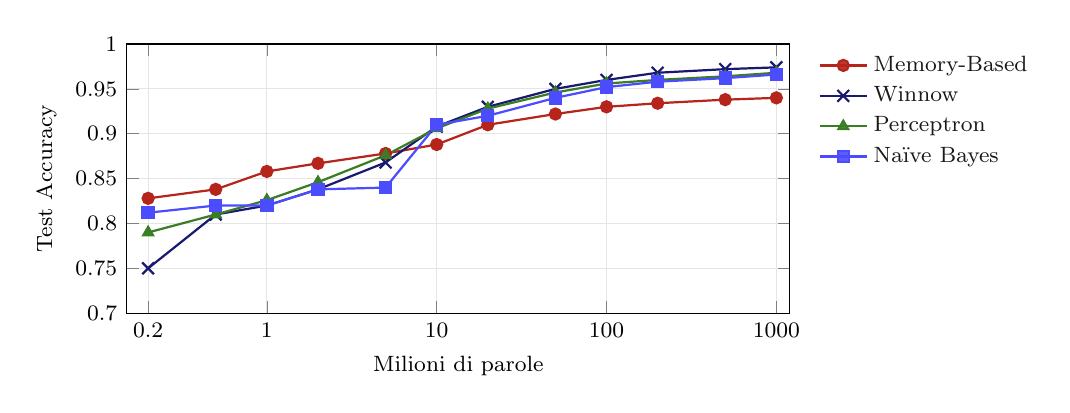
\begin{tikzpicture}
\begin{axis}[
    width=10cm, height=5cm,
    xmode=log,
    xmin=0.15, xmax=1200,
    ymin=0.70, ymax=1.00,
    xlabel={Milioni di parole},
    ylabel={Test Accuracy},
    grid=major, grid style=gray!20,
    legend pos=outer north east,
    legend style={font=\footnotesize, cells={anchor=west}, 
                  legend columns=1, draw=none, fill=white, fill opacity=0.9},
    legend cell align={left},
    xtick={0.2, 1, 10, 100, 1000},
    xticklabels={0.2, 1, 10, 100, 1000},
    ytick={0.70,0.75,0.80,0.85,0.90,0.95,1.00},
    tick label style={font=\footnotesize},
    label style={font=\footnotesize}
]
\addplot[color=BrickRed, mark=*, thick] coordinates {
    (0.2,0.828)(0.5,0.838)(1,0.858)(2,0.867)(5,0.878)
    (10,0.888)(20,0.910)(50,0.922)(100,0.930)(200,0.934)(500,0.938)(1000,0.940)
};
\addlegendentry{Memory-Based}

\addplot[color=MidnightBlue, mark=x, mark size=3pt, thick] coordinates {
    (0.2,0.750)(0.5,0.810)(1,0.820)(2,0.838)(5,0.868)
    (10,0.908)(20,0.930)(50,0.950)(100,0.960)(200,0.968)(500,0.972)(1000,0.974)
};
\addlegendentry{Winnow}

\addplot[color=OliveGreen, mark=triangle*, thick] coordinates {
    (0.2,0.790)(0.5,0.810)(1,0.826)(2,0.846)(5,0.876)
    (10,0.906)(20,0.928)(50,0.946)(100,0.956)(200,0.960)(500,0.964)(1000,0.968)
};
\addlegendentry{Perceptron}

\addplot[color=blue!70, mark=square*, thick] coordinates {
    (0.2,0.812)(0.5,0.820)(1,0.820)(2,0.838)(5,0.840)
    (10,0.910)(20,0.920)(50,0.940)(100,0.952)(200,0.958)(500,0.962)(1000,0.966)
};
\addlegendentry{Na\"ive Bayes}

\end{axis}
\end{tikzpicture}
\end{center}



\subsection{Rappresentatività del campione}
I dati non devono essere solo tanti -- devono \textbf{rappresentare il problema reale}:

\begin{itemize}
    \item \textbf{PIL pro capite}: se il training set include solo paesi ricchi o solo paesi poveri, il modello non rappresenterà la realtà globale e avrà prestazioni scarse agli estremi.
    \item \textbf{Classificazione di immagini}: se si addestra il modello solo con foto di gatti, non saprà riconoscere cani o scoiattoli.
    \item \textbf{Studi demografici}: l'età dei campioni deve rispecchiare l'obiettivo. Per studi alimentari serve la popolazione totale; per studi sulla digitalizzazione ha senso restringersi a un range (es.\ 6--50 anni). I paesi asiatici o africani hanno piramidi demografiche con molti giovani e pochi anziani -- questo influisce profondamente sulla composizione del dataset.
\end{itemize}

\begin{exbox}[L'aneddoto di Gallup vs.\ Literary Digest (1936)]
\textbf{Literary Digest}: condusse un sondaggio con 10 milioni di persone campionate da elenchi telefonici e abbonamenti a riviste. Predisse Landon vincitore con il 57\% dei voti. Roosevelt vinse con il 62\%. Errore: \textbf{sampling bias} -- il campione non era rappresentativo della popolazione.

\textbf{George Gallup}: indovinò il risultato con soli 50\.000 elettori, ma divisi  per età e classe sociale. La \textbf{qualità della rappresentatività} contava più della quantità.
\end{exbox}

\section{I limiti dei modelli: il problema della non-linearità}
La regressione lineare assume dati con andamento rettilineo. Cosa succede se usiamo un modello non lineare (polinomio di grado elevato) per essere più precisi?

\begin{center}
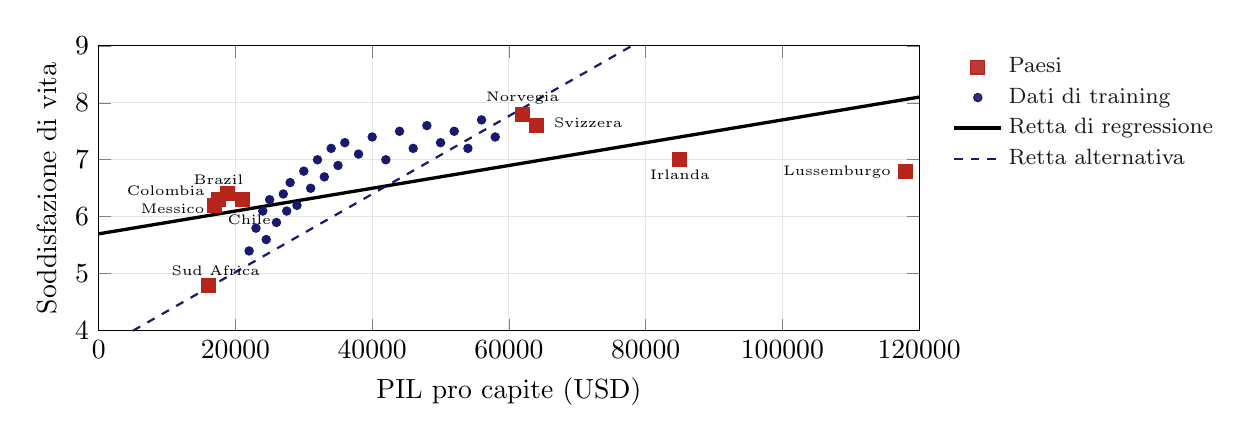
\begin{tikzpicture}
\begin{axis}[
    width=12cm, height=5.2cm,
    xlabel={PIL pro capite (USD)},
    ylabel={Soddisfazione di vita},
    xmin=0, xmax=120000, ymin=4, ymax=9,
    grid=major, grid style={gray!20},
    legend pos=outer north east,
    legend style={font=\footnotesize, cells={anchor=west}, 
                  legend columns=1, draw=none, fill=white, fill opacity=0.9},
    legend cell align={left},
    ytick={4,5,6,7,8,9},
    xtick={0,20000,40000,60000,80000,100000,120000},
    xticklabels={0,20000,40000,60000,80000,100000,120000},
    scaled x ticks=false,
    clip=false
]

% Quadrati rossi (9 paesi)
\addplot[only marks, mark=square*, mark size=2.5pt, BrickRed] coordinates {
    (16000,4.8)   % Sud Africa
    (17000,6.2)   % Colombia
    (17500,6.3)   % Brazil
    (18800,6.4)   % Messico
    (21000,6.3)   % Chile
    (62000,7.8)   % Norvegia
    (64000,7.6)   % Svizzera
    (85000,7.0)   % Irlanda
    (118000,6.8)  % Lussemburgo
};
\addlegendentry{Paesi}

% Pallini blu (28 punti casuali tra 21000 e 58000)
\addplot[only marks, mark=*, mark size=1.5pt, MidnightBlue] coordinates {
    (22000,5.4)(23000,5.8)(24000,6.1)(24500,5.6)(25000,6.3)
    (26000,5.9)(27000,6.4)(27500,6.1)(28000,6.6)(29000,6.2)
    (30000,6.8)(31000,6.5)(32000,7.0)(33000,6.7)(34000,7.2)
    (35000,6.9)(36000,7.3)(38000,7.1)(40000,7.4)(42000,7.0)
    (44000,7.5)(46000,7.2)(48000,7.6)(50000,7.3)(52000,7.5)
    (54000,7.2)(56000,7.7)(58000,7.4)
};
\addlegendentry{Dati di training}

% Retta di regressione principale
\addplot[
    domain=0:120000,
    samples=2,
    very thick,
    black
]
{5.7 + 0.00002*x};
\addlegendentry{Retta di regressione}

% Retta alternativa tratteggiata
\addplot[
    domain=5000:78000,
    samples=2,
    thick,
    MidnightBlue,
    dashed
]
{4 + 0.0000685*(x-5000)};
\addlegendentry{Retta alternativa}

% Nomi dei paesi (font minuscolo)
\node[font=\tiny, anchor=south east] at (axis cs:25000,4.8)  {Sud Africa};
\node[font=\tiny, anchor=south]     at (axis cs:9800,6.2)  {Colombia};
\node[font=\tiny, anchor=south]     at (axis cs:17500,6.4)  {Brazil};
\node[font=\tiny, anchor=north]     at (axis cs:10800,6.4)  {Messico};
\node[font=\tiny, anchor=north]     at (axis cs:22000,6.2)  {Chile};
\node[font=\tiny, anchor=south]     at (axis cs:62000,7.8)  {Norvegia};
\node[font=\tiny, anchor=south east] at (axis cs:78000,7.4)  {Svizzera};
\node[font=\tiny, anchor=north]     at (axis cs:85000,7.0)  {Irlanda};
\node[font=\tiny, anchor=south]     at (axis cs:108000,6.5) {Lussemburgo};

\end{axis}
\end{tikzpicture}
\end{center}


\begin{itemize}
    \item \textbf{Quadrati rossi a sinistra}: PIL basso ma soddisfazione sorprendentemente alta (es.\ Brasile).
    \item \textbf{Quadrati rossi a destra}: PIL alto ma soddisfazione più bassa delle aspettative (es.\ Lussemburgo).
    \item \textbf{Retta tratteggiata blu}: addestrata solo sui dati parziali (pallini blu). È errata per i paesi anomali -- il modello si è \emph{specializzato} su un sottoinsieme e non sa gestire le eccezioni.
    \item \textbf{Retta nera continua}: addestrata su tutti i dati. È una retta di compromesso, passa meno vicino ai pallini, ma fa previsioni più realistiche anche per i casi anomali.
\end{itemize}

Questo è l'essenza del problema \textbf{overfitting vs.\ underfitting}.

\section{Overfitting vs.\ Underfitting}
\label{sec:overfit}
\begin{defbox}[La metafora degli studenti]
Tre alunni si preparano per un esame:
\begin{enumerate}
    \item \textbf{Primo}: impara tutti gli esercizi a memoria senza capire.
    \item \textbf{Secondo}: non studia nulla.
    \item \textbf{Terzo}: fa gli esercizi richiesti ma capisce la \emph{regola generale}.
\end{enumerate}
Il giorno della verifica, il terzo prenderà il voto più alto. Il primo, di fronte a un problema leggermente diverso da quelli memorizzati, andrà male. Il secondo andrà male sempre.
\end{defbox}


\begin{center}
\begin{tikzpicture}
\begin{groupplot}[
    group style={group size=3 by 1, horizontal sep=1.8cm},
    width=5.2cm, height=4.8cm,
    xmin=0, xmax=10, ymin=-0.5, ymax=7,
    xtick=\empty, ytick=\empty,
    title style={font=\small\bfseries},
    axis lines=left,
    axis line style={gray!50, thin}
]

\nextgroupplot[title={Overfitting}]
\addplot[only marks, mark=*, mark size=1.6pt, color=Goldenrod!85!black] coordinates {
    (0.5,5.4)(1,4.1)(1.5,3.1)(2,3.3)(2.5,2.1)(3,1.9)(3.5,1.7)
    (4,0.8)(4.5,1.3)(5,0.9)(5.5,1.0)(6,1.6)(6.5,1.3)(7,2.3)
    (7.5,2.6)(8,3.0)(8.5,4.0)(9,4.2)
};
\addplot[domain=0.4:9.4, samples=300, very thick, MidnightBlue]
    {0.2*(x-5)^2 + 1
     + 1.8*sin(deg(3.5*x))*exp(-0.08*(x-5)^2)
     + 0.9*cos(deg(2.2*x))*exp(-0.12*(x-3)^2)};
\node[font=\scriptsize, text=MidnightBlue, align=center]
    at (axis cs:5,-0.3) {Modello troppo complesso};

\nextgroupplot[title={Good fit}]
\addplot[only marks, mark=*, mark size=1.6pt, color=Goldenrod!85!black] coordinates {
    (0.5,5.4)(1,4.1)(1.5,3.1)(2,3.3)(2.5,2.1)(3,1.9)(3.5,1.7)
    (4,0.8)(4.5,1.3)(5,0.9)(5.5,1.0)(6,1.6)(6.5,1.3)(7,2.3)
    (7.5,2.6)(8,3.0)(8.5,4.0)(9,4.2)
};
\addplot[domain=0:10, samples=80, very thick, OliveGreen]
    {0.2*(x-5)^2 + 1};
\node[font=\scriptsize, text=OliveGreen, align=center]
    at (axis cs:5,-0.3) {Buona generalizzazione};

\nextgroupplot[title={Underfitting}]
\addplot[only marks, mark=*, mark size=1.6pt, color=Goldenrod!85!black] coordinates {
    (0.5,5.4)(1,4.1)(1.5,3.1)(2,3.3)(2.5,2.1)(3,1.9)(3.5,1.7)
    (4,0.8)(4.5,1.3)(5,0.9)(5.5,1.0)(6,1.6)(6.5,1.3)(7,2.3)
    (7.5,2.6)(8,3.0)(8.5,4.0)(9,4.2)
};
\addplot[domain=0:10, samples=2, very thick, BrickRed]
    {0.06*x + 2.0};
\node[font=\scriptsize, text=BrickRed, align=center]
    at (axis cs:5,-0.3) {Modello troppo semplice};

\end{groupplot}
\end{tikzpicture}
\end{center}


\begin{itemize}
    \item \textbf{Overfitting (Lo studente che impara a memoria)}: il modello memorizza i dettagli e il ``rumore'' del training set invece di imparare lo schema generale. Ottima corrispondenza in training, errore altissimo sui nuovi dati in test. Causa tipica: modello troppo complesso rispetto alla quantità e alla rumorosità dei dati.

    Soluzioni:
    \begin{itemize}
        \item \textbf{Regolarizzazione} (L1/Lasso, L2/Ridge): inserisce vincoli matematici per evitare grandi oscillazioni della curva e mantenere i parametri piccoli e semplici.
        \item Raccogliere più dati di training.
        \item Ridurre la complessità del modello (meno parametri, meno feature).
        \item \emph{Early stopping}: interrompere l'addestramento quando l'errore sul validation set smette di migliorare.
    \end{itemize}

    \item \textbf{Underfitting (Lo studente che non studia)}: il modello è troppo semplice per catturare la struttura dei dati. Errori elevati sia in training che in test.

    Soluzioni:
    \begin{itemize}
        \item Scegliere un modello più espressivo (più parametri, architettura più complessa).
        \item Feature engineering: aggiungere feature più informative.
        \item Ridurre la regolarizzazione se è troppo forte.
        \item Aumentare il numero di epoche di training.
    \end{itemize}
\end{itemize}

\textbf{L'Errore di Generalizzazione} è proprio la misura dell'errore che il modello commette quando affronta nuovi dati (testing set) estratti dalla stessa distribuzione dei dati usati nel training.


\section{Divisione del dataset e Cross-Validation}
\subsection{Suddivisione standard (2 vie)}
\begin{itemize}
    \item \textbf{Training set} ($\sim$80\%): per addestrare il modello (trovare $\theta_0, \theta_1$, i pesi, \ldots).
    \item \textbf{Test set} ($\sim$20\%): per valutare quanto il modello funziona su dati mai visti.
\end{itemize}

\subsection{Suddivisione industriale (3 vie)}
\begin{center}
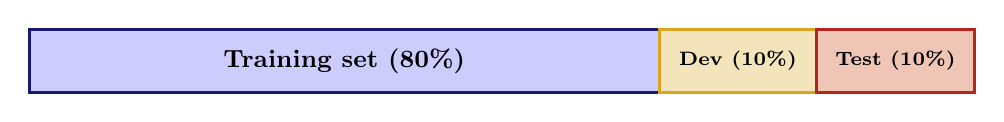
\begin{tikzpicture}[font=\small]
\draw[fill=blue!20, draw=MidnightBlue, very thick]
    (0,0) rectangle (8,0.8) node[midway] {\bfseries Training set (80\%)};
\draw[fill=Goldenrod!30, draw=Goldenrod, very thick]
    (8,0) rectangle (10,0.8) node[midway, font=\scriptsize] {\bfseries Dev (10\%)};
\draw[fill=BrickRed!20, draw=BrickRed, very thick]
    (10,0) rectangle (12,0.8) node[midway, font=\scriptsize] {\bfseries Test (10\%)};
\end{tikzpicture}
\end{center}

\begin{itemize}
    \item \textbf{Training set} (80\%): addestramento del modello.
    \item \textbf{Dev / Validation set} (10\%): usato \emph{in corso d'opera} per confrontare modelli diversi e mettere a punto gli iperparametri -- senza toccare il test set.
    \item \textbf{Test set} (10\%): usato \emph{solo alla fine}, una volta sola, per la validazione assoluta del modello scelto.
\end{itemize}

\subsection{Cross-Validation (Convalida Incrociata)}

Se il dataset ha 70\,000 immagini, le dividiamo in 7 ``pacchetti'' da 10\,000 (\emph{fold}). A ogni iterazione si usano 60\,000 per il training e 10\,000 per il test, ruotando il fold di test. Si ottengono 7 valori di precisione; la \textbf{media} di questi 7 valori è la stima finale del modello.

\begin{center}
\begin{tikzpicture}[font=\scriptsize, node distance=0.15cm]
\foreach \i in {1,...,7} {
    \pgfmathsetmacro{\xstart}{(\i-1)*1.35}
    \pgfmathparse{\i==1 ? 1 : 0}
    \ifnum\i=1
        \draw[fill=BrickRed!30, draw=BrickRed, thick]
            (\xstart,0) rectangle (\xstart+1.2,0.55) node[midway]{\textbf{Test}};
    \else
        \draw[fill=blue!15, draw=MidnightBlue, thick]
            (\xstart,0) rectangle (\xstart+1.2,0.55) node[midway]{Train};
    \fi
}
\node[right] at (9.6, 0.28) {$\to$ Acc$_1$};

\foreach \i in {1,...,7} {
    \pgfmathsetmacro{\xstart}{(\i-1)*1.35}
    \ifnum\i=2
        \draw[fill=BrickRed!30, draw=BrickRed, thick]
            (\xstart,-0.75) rectangle (\xstart+1.2,-0.2) node[midway]{\textbf{Test}};
    \else
        \draw[fill=blue!15, draw=MidnightBlue, thick]
            (\xstart,-0.75) rectangle (\xstart+1.2,-0.2) node[midway]{Train};
    \fi
}
\node[right] at (9.6, -0.47) {$\to$ Acc$_2$};

\node at (4.75, -1.1) {\ldots};
\node[right] at (9.6, -1.1) {\ldots};

\foreach \i in {1,...,7} {
    \pgfmathsetmacro{\xstart}{(\i-1)*1.35}
    \ifnum\i=7
        \draw[fill=BrickRed!30, draw=BrickRed, thick]
            (\xstart,-1.6) rectangle (\xstart+1.2,-1.05) node[midway]{\textbf{Test}};
    \else
        \draw[fill=blue!15, draw=MidnightBlue, thick]
            (\xstart,-1.6) rectangle (\xstart+1.2,-1.05) node[midway]{Train};
    \fi
}
\node[right] at (9.6, -1.32) {$\to$ Acc$_7$};

\node[align=center, font=\small] at (4.75, -2.1)
    {Stima finale $= \dfrac{\text{Acc}_1 + \text{Acc}_2 + \cdots + \text{Acc}_7}{7}$};
\end{tikzpicture}
\end{center}

\begin{itemize}
    \item \textbf{Vantaggio}: evita bias involontari (es.\ escludere donne, anziani o un gruppo demografico dal test per puro caso); garantisce che il modello si alleni su diverse combinazioni di dati.
    \item \textbf{Svantaggio}: aumenta il costo computazionale di un fattore $k$ (qui 7). La variante \textbf{Stratified $k$-fold} mantiene le proporzioni delle classi in ogni fold -- fondamentale per dataset sbilanciati.
\end{itemize}

\section{Iperparametri vs.\ parametri}

\begin{itemize}
    \item \textbf{Parametri}: appresi automaticamente durante il training (es.\ $\theta_0, \theta_1$ nella regressione lineare, i pesi delle reti neurali). Il modello li ottimizza minimizzando la funzione di costo.
    \item \textbf{Iperparametri}: scelti \emph{prima} del training e rimangono fissi durante l'addestramento (es.\ $k$ in kNN, \texttt{max\_depth} negli alberi decisionali, il \emph{learning rate}, la forza della regolarizzazione). Non vengono appresi dall'algoritmo, ma impostati dal progettista.
\end{itemize}

La ricerca degli iperparametri migliori si fa su un \textbf{validation set}, usando tecniche come:
\begin{itemize}
    \item \textbf{Grid search}: si prova ogni combinazione di una griglia di valori pre-definiti.
    \item \textbf{Random search}: si campionano combinazioni casuali -- spesso più efficiente della grid search per spazi ad alta dimensionalità.
    \item \textbf{Bayesian optimization}: usa un modello probabilistico per guidare la ricerca verso le regioni più promettenti.
\end{itemize}

\section{No Free Lunch Theorem}

\begin{thmbox}[Teorema No Free Lunch (Wolpert, 1996)]
Mediando su tutti i possibili problemi, qualsiasi coppia di algoritmi di apprendimento ha la stessa prestazione attesa. \textbf{Non esiste un algoritmo universalmente migliore per tutti i problemi.}

In pratica si parte testando alcune famiglie ragionevoli in base al problema (baseline lineare, Random Forest, Gradient Boosting, MLP) e si confrontano in cross-validation.
\end{thmbox}

\section{Conclusioni sul Machine Learning}

Il successo di un sistema ML dipende primariamente da:
\begin{enumerate}
    \item \textbf{Qualità e quantità dei dati}: la collezione e pulizia dei dati rappresenta tipicamente il 70--80\% del lavoro reale di un progetto.
    \item \textbf{Feature engineering}: scegliere le colonne/attributi giusti fa spesso più differenza della scelta dell'algoritmo.
    \item \textbf{Scelta della famiglia di modelli}: adeguata al problema e alla quantità di dati disponibili.
    \item \textbf{Rigorosa valutazione}: training/validation/test set ben separati, cross-validation, monitoraggio in produzione.
\end{enumerate}